The first part of the work will be to observe a number of handovers between humans for a set of objects and try to categorise the observed handovers into different classes. In a second part each object will then be assigned a class that we train a machine to return when given an image.

Seeing how we do not have any labels for the handovers, but still want to train a model that outputs some defined class for how the object should be handed over, we will be using a semi-supervised approach in this project. By first applying an unsupervised learning algorithm to categorise and create classes of handovers that are later used as output through supervised learning.

\section{Categorisation of handovers}

\subsection{Collection of data}

For this purpose a number of voluteers were asked to be recorded while handing over a set of objects between each other, using a \emph{Kinect v2} the \textcite{libfreenect2} software library. Even though the camera used supports depth images, only two-dimensional data will be used in these part, i.e we will only use the color images recorded. A total of 11 people who already knew each other from before volunteered (including myself) for this task.  Pairs of volunteers were permutted to try and make givers adapt to different recievers. 15 objects were used in the recordings including: \emph{kitchen knife, hammer, screwdriver, brush, pen, scissors, bottle, cup, pitcher, glass, ball, tube, box, can, scalpel}. Instructions for handing over the objects were given prior to recordings as to make sure participants gave the object in a manner that the reciever can used the object straight away, for example give the hammer handle first in a manner that the next person can start hammering directly without requiring a switch of grip after recieving, or a cup is to handed handle first so the person can start drinking right away. For objects that might contain liquids the participants were asked to imagine that these objects were filled while handing them over between each other. Also as to make sure the dataset did not contain too much deviations considering the grasp some instructions were given concerning region were to grasp, for example that the giver grasps the bottle in the top half. The regions were chosen by myself with in mind for optimization for the reciever when given the object.

In order to extract data from the recorded frames about the objects we need to detect the objects themselves. Object detection is a very difficult part of computer vision and there are many different methods, where some are more robust than others, to do so. To help with this part to make data extraction easier we will be using AprilTags. AprilTags can be compared to QR-codes that are printed out on small papers and fastened onto the objects. With the help of their software library we can easily track the objects in the recorded material by getting the position of the four corners of the tag, and its center, which enables us to estimate such things as pose of the object. More can be learned about AprilTags at \parencite{AprilTags}.

For each object we manually first create a reference image with its ground truth and from this image we also generate a binary mask. Figure \ref{fig:objects_montage} shows the reference images created and figure \ref{fig:masks_montage} show their binary masks. These images were created using the \textcite{GIMP} - GIMP. With the help of the AprilTags we can compute a Homography matrix that would warp the tag (and object) in the reference image to the one located in the frame with the detected object. The binary mask of the image is transformed using the computed Homography matrix and applied over the scene to extract only the entire object itself, and with this we can estimate the grasping region. The image of the found object is segmentated by color, skin color more precisely in this case, and a contour expressed as rotated rectangle is calculated around the largest region found which represents our grasping region. Skin color is a quick way of segmentating and finding grasp region as the color of skin is quite different from the colors of the objects, but the method is not too robust in covering many different people as the color can vary quite a lot from person to person. The setting for skin color had to therefore be tweaked manually depending on the participant.

\begin{figure}
	\centering
	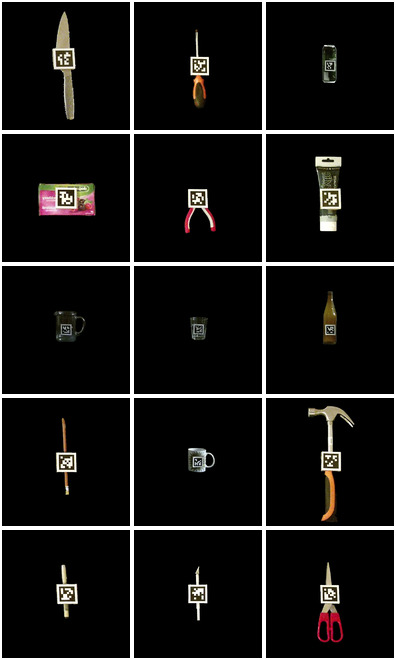
\includegraphics[width=\textwidth]{img/methods/objects.jpg}
	\caption{Ground truth images of the objects used with an AprilTag fastened to them}
	\label{fig:objects_montage}
\end{figure}

\begin{figure}
	\centering
	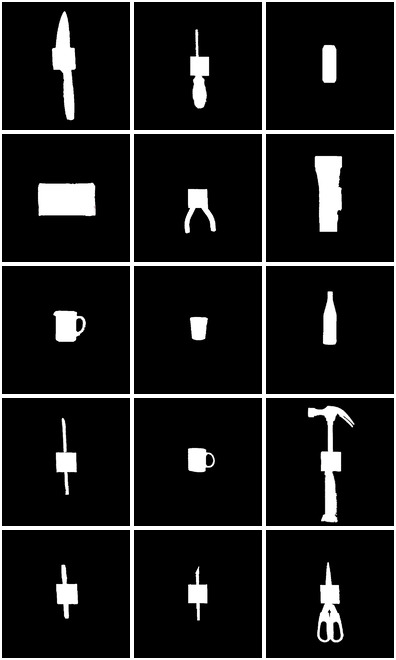
\includegraphics[width=\textwidth]{img/methods/masks.jpg}
	\caption{Binary mask of each object}
	\label{fig:masks_montage}
\end{figure}

One recording session consists from one pair of volunteers, the giver has handed over all objects in the set to the reciever. During the recording the application is continuously recording, creating a large number frames that are not of interest. In this project we only interest ourselves for the actual moment that the giver holds out the object ready for the reciever to take it, which requires some post-processing of the frames. A first step is to create a Region of Interest (ROI) which we will concentrate on searching for objects. Our ROI is arbitrarely set to the middle of the frame and large enough to see the entire object. When a tag is detected within the the ROI we flag this frame a handover moment and store the features of the handover. This is unfortunately not enough because we might be flagging frames where the reciever is holding the object after taking it, or maybe both are holding it but the system detects the reciever's hand as the largest grasping region. The methods explained above might also be incorrect as the grasping region was incorrectly detected. Manual filtering was later applied to images that were flagged as handover moments and to make sure they were correct ones and that the data extracted was correct.

\begin{figure}
	\centering
	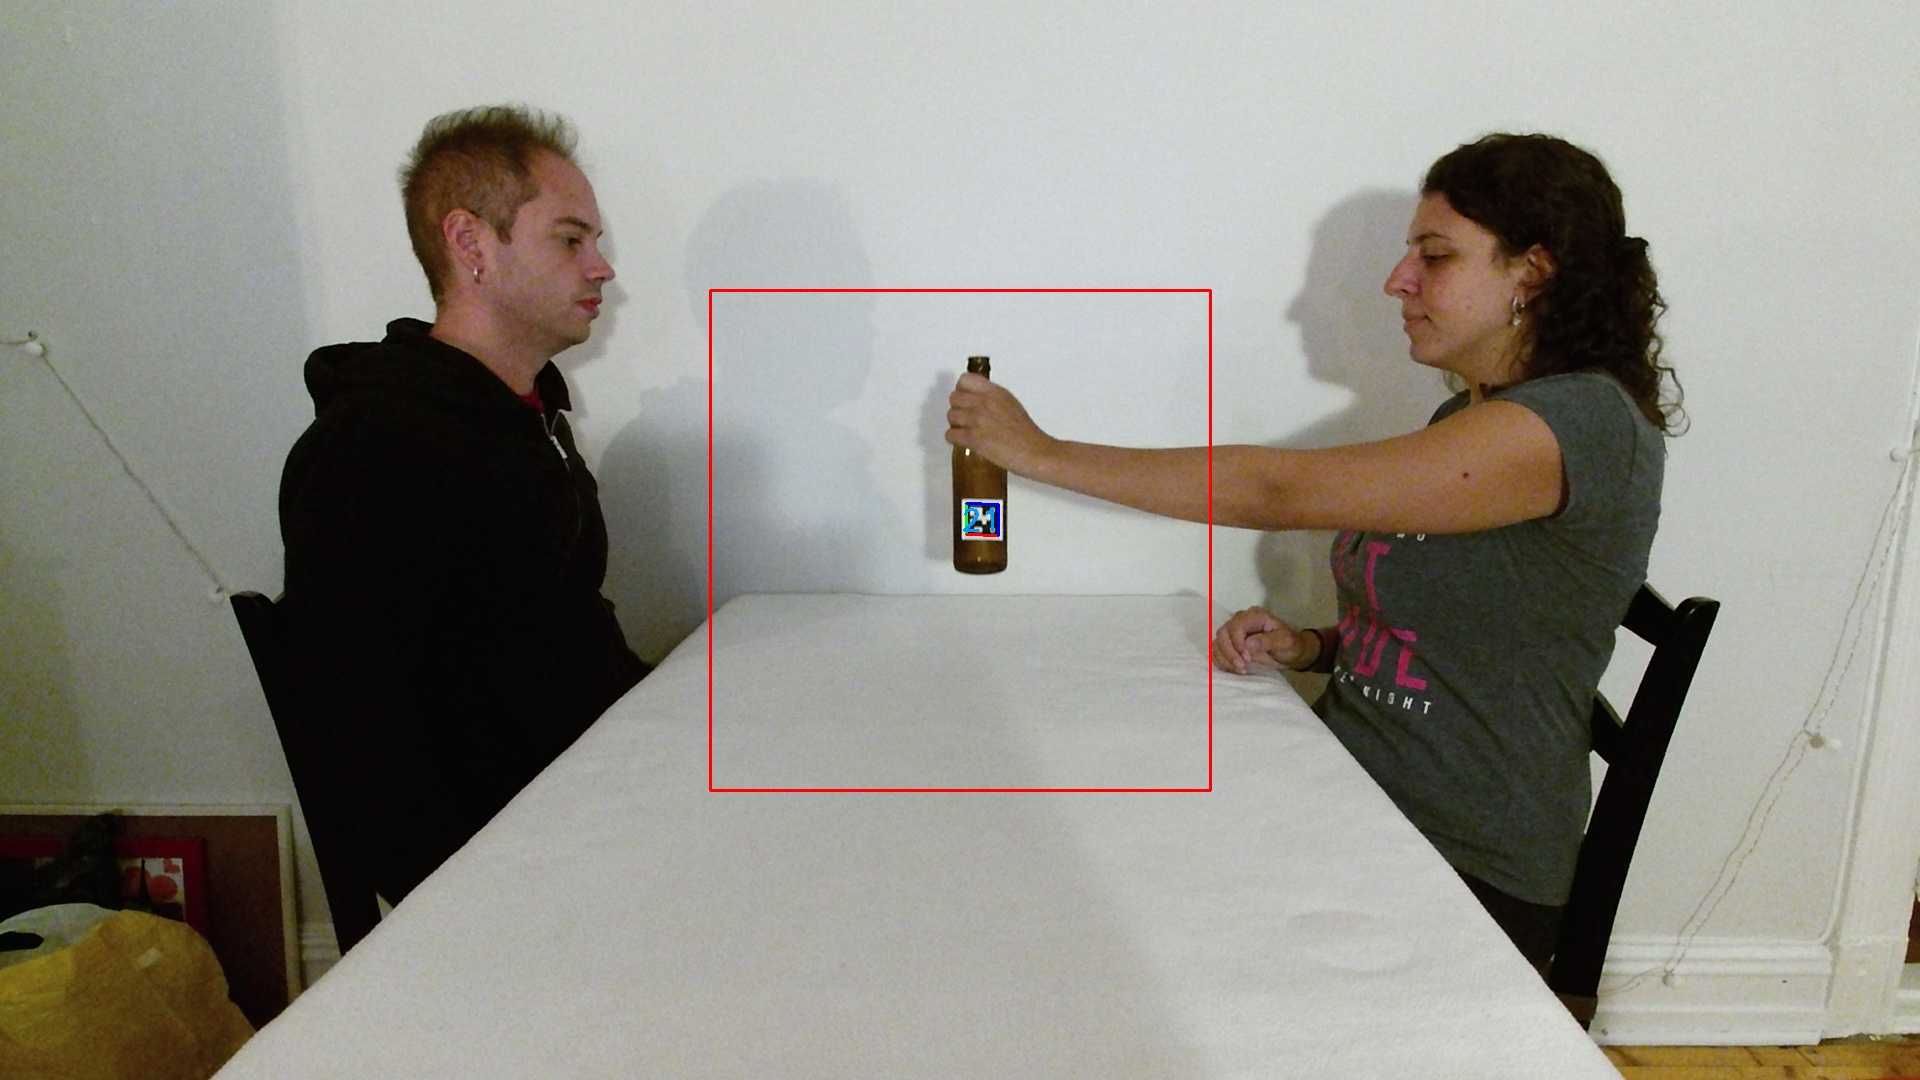
\includegraphics[width=\textwidth]{img/methods/handovers/bottle_frame.jpg}
	\caption{}
	\label{fig:handover_bottle}
\end{figure}

\begin{figure}
	\centering
	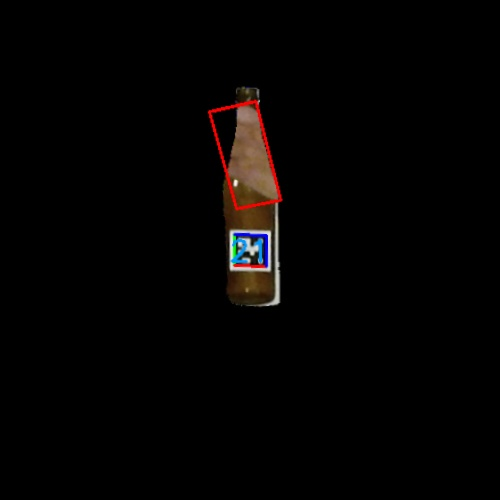
\includegraphics[width=0.5\textwidth]{img/methods/handovers/bottle_masked.jpg}
	\caption{}
	\label{fig:handover_bottle_masked}
\end{figure}

\begin{figure}
	\centering
	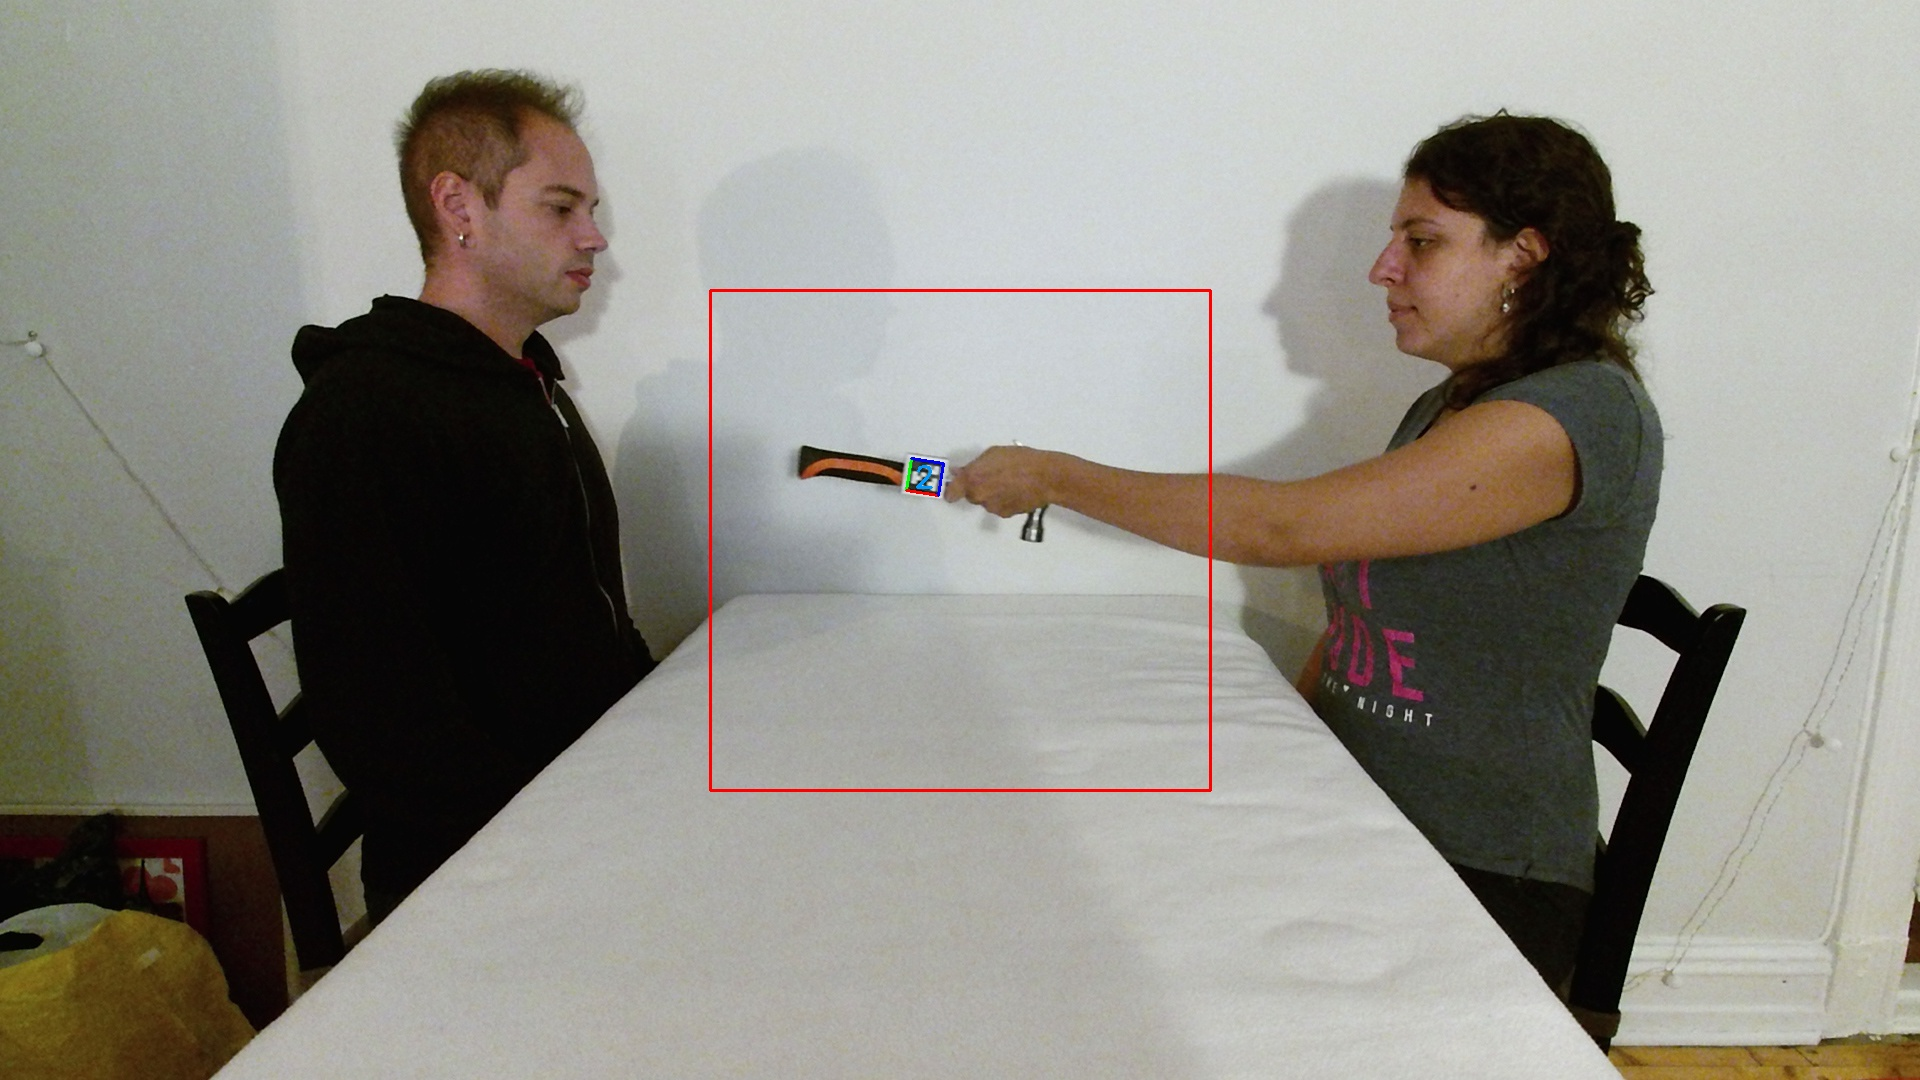
\includegraphics[width=\textwidth]{img/methods/handovers/hammer_frame.jpg}
	\caption{}
	\label{fig:handover_hammer}
\end{figure}

\begin{figure}
	\centering
	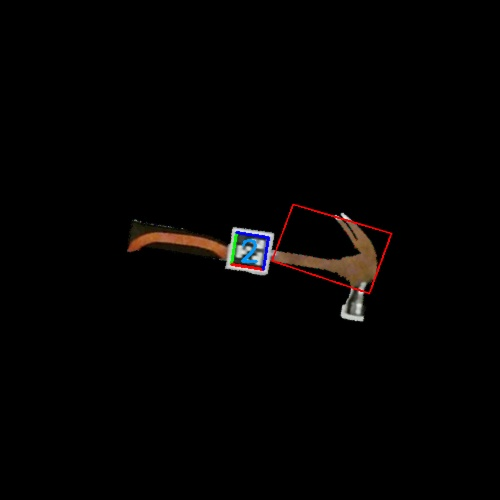
\includegraphics[width=0.5\textwidth]{img/methods/handovers/hammer_masked.jpg}
	\caption{}
	\label{fig:handover_hammer_masked}
\end{figure}

\begin{figure}
	\centering
	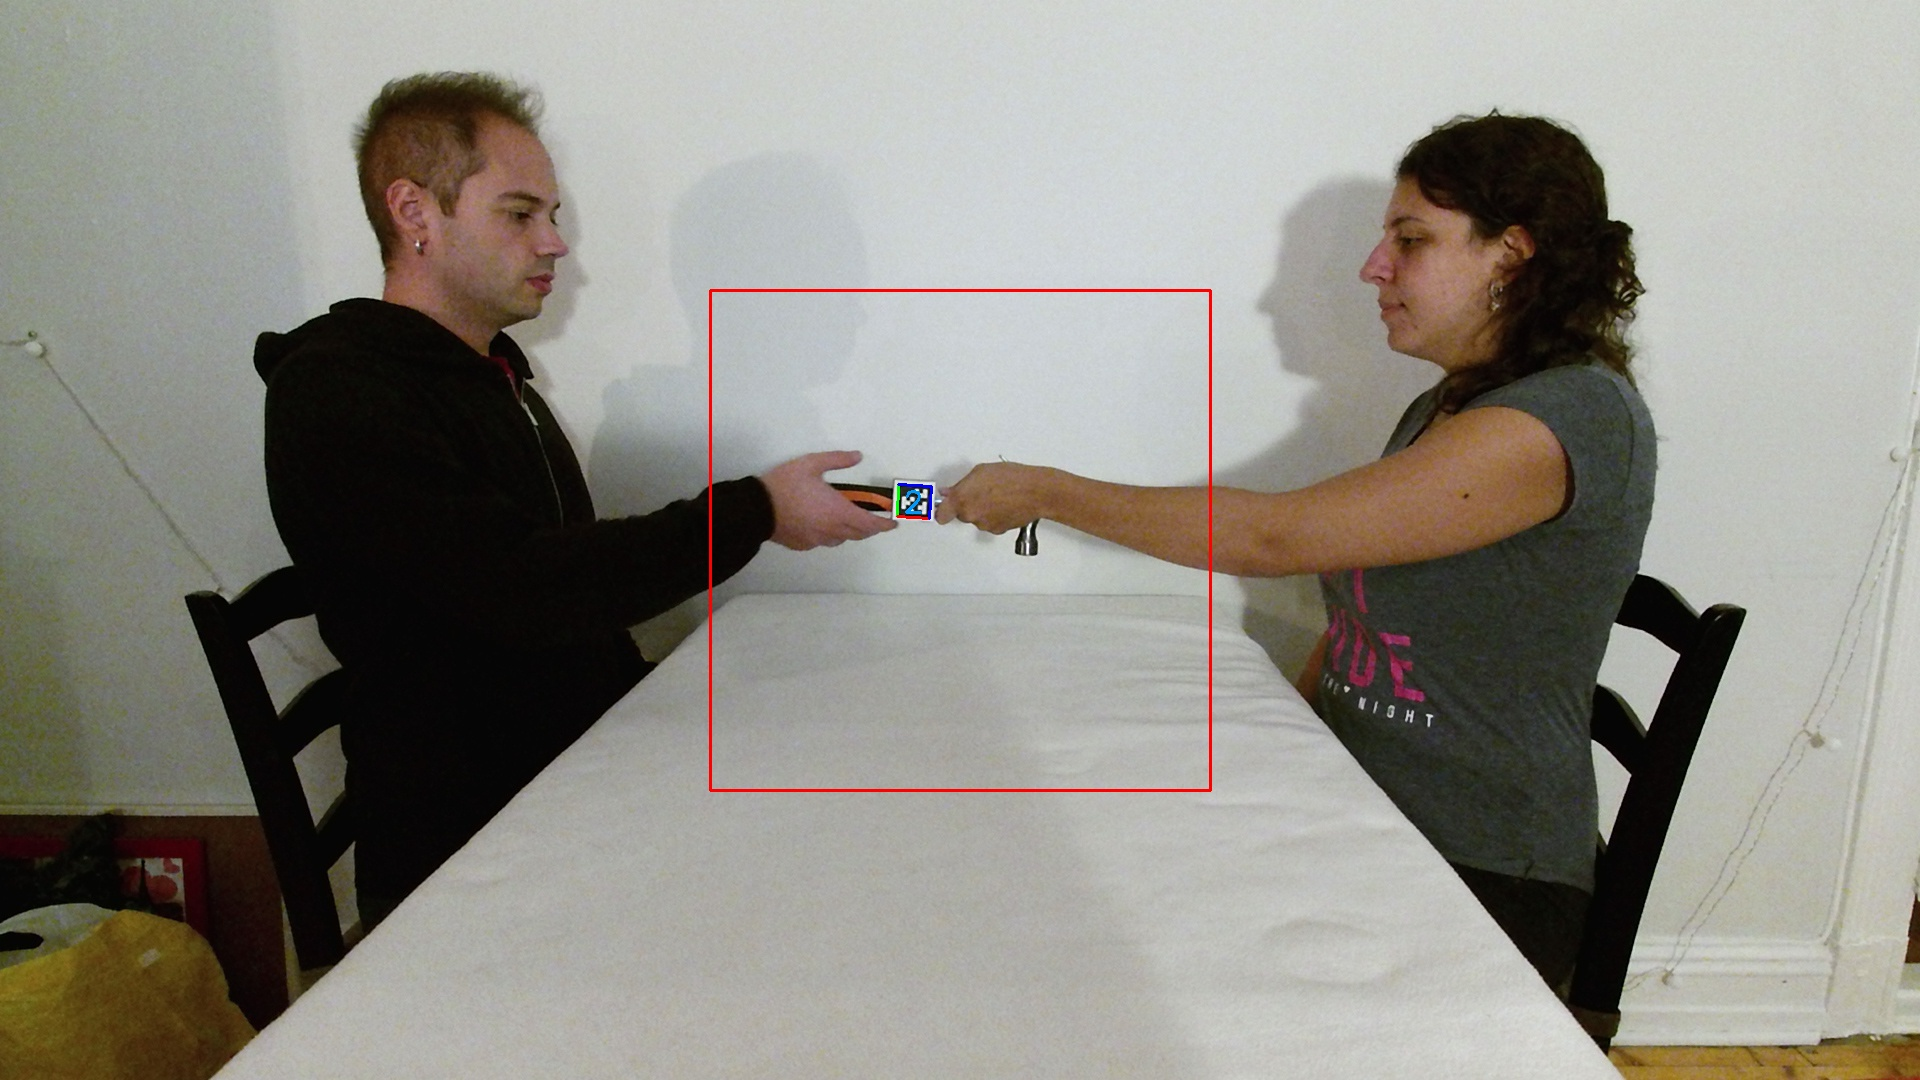
\includegraphics[width=\textwidth]{img/methods/handovers/incorr_frame.jpg}
	\caption{}
	\label{fig:handover_incorr}
\end{figure}

\begin{figure}
	\centering
	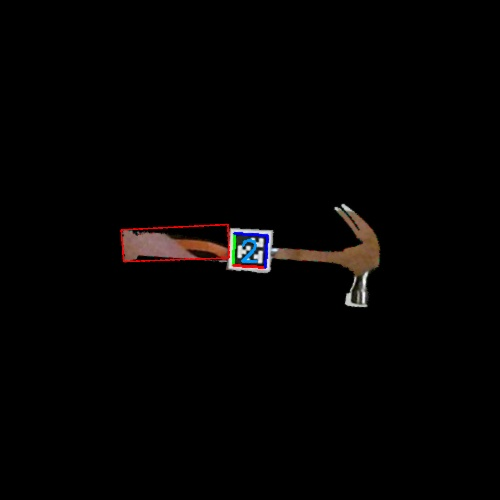
\includegraphics[width=0.5\textwidth]{img/methods/handovers/incorr_mask.jpg}
	\caption{}
	\label{fig:handover_incorr_masked}
\end{figure}


\subsection{Clustering by handover features}

After observing a number of handovers betweens humans, a first step is to try and categorise these handovers into different classes that can be applied for the objects. As we do not have any labels, or even unsure how many different categories of handovers we have recorded, we will attempt at clustering using an unsupervised learning algorithm by the features that we have extracted from the recorded material.

\subsubsection{K-Means}

For the purpose of categorizing the handover samples we will be using the \emph{k-means} algorithm. K-means is an algorithm that attempts to classify a number of observations into \emph{k} number of clusters. The algorithm starts by creating \emph{k} number of centroids for each cluster and assigning our samples to the centroid within shortest distance. The algorithm iteratively then updates the centroids to become the mean of the samples assigned to it, and then re-assigns all samples depending on the new centroids. This is repeated either a fixed number of times or until the algorithm converges minimizing the sum of squares within the clusters.

\subsubsection{Principle component analysis (PCA)}

A challenge that presents itself using clustering algorithms is choosing what features are to be used for the purpose and how many clusters should we create. We will be using \emph{Principle component analysis} (PCA) to evaluate which features that are to be used to define each cluster. Ideally we use the smallest number of features possible, but also the ones that create the most distinct clusters, which PCA will help us with. Before using techniques such as PCA to minimize the amount of features that are needed to cluster we will try to define what features matter in a handover and deduct them from the data we have, as well as trying to redefine some features in a more compressed matter.

\subsubsection{Extracting features}

As we mentioned we are able to extract the homography matrix the grasping region expressed as a rotated rectange from the recorded data. From these we can derive a number of features that might be of interest to classify a handover. A homography matrix \(H\) is a 3x3 matrix with a total of nine values which creates quite a few features if we would try and cluster on it. Instead we can use it to calculate a rotation of the object, we discard the translation information in the matrix as we are only interested in the end pose of the object. As we are only working with two-dimensional data we will use the rotation on the z-axis. Using the homography we can calculate a rotation matrix from which we can derive the angle. Using the following Python, code with the help of the OpenCV library we compute a rotation matrix \(R\) (taken from \parencite{OpenCVHomographyDemo}). Using the rotation matrix we can compute the angle \(\theta_Z\) as \(\theta_Z = \arctan(R_{1,0} / R_{0,0})\).

\begin{lstlisting}[language=Python]
norm = np.sqrt(np.sum(H[:,0] ** 2))
H /= norm
c1 = H[:, 0]
c2 = H[:, 1]
c3 = np.cross(c1, c2)

R = np.zeros((3, 3), dtype=np.float64)
for i in range(3):
	R[i, :] = [c1[i], c2[i], c3[i]]
w, u, t = cv2.SVDecomp(R)
return np.dot(u, t)
\end{lstlisting}

Next we can compute a center of mass for the object using it's contour's moments, easily extracted from it's binary mask. The following formula gives us the center. \textcolor{red}{write about moments and correct formula for center}

\[
	center = \frac{M_x}{M}, \frac{M_y}{M}
\]

We can then extract the distance between center of mass of the object and the center of the grasping region as a feature. It also enables us to create a unit vector from the center of mass of the object towards the grasping region. A vector in two dimensions would be expressed with two values, but we can summarize this in one value by instead calculating the angle using \(\tan(\theta) = \sqrt{x^2 + y^2}\). Lastly we can compute the ratio of the area covered by the grasp by the area of the object \(A = \frac{area(Grasp)}{area(Object}\).

To summarize we can extract the following features: \textcolor{red}{make the below lists better}
\begin{itemize}
	\item Rotation of object in z-axis, extracted from the homography matrix of the AprilTag.
	\item Distance between center of mass of the object and the center of the grasping region.
	\item Angle between the two mentioned centers.
	\item Ratio of area of the grasping region by the area of object.
\end{itemize}

On top of these we still have:
\begin{itemize}
	\item Width of grasp region
	\item Height of grasp region
	\item Angle of grasp region
	\item Center of grasp region
	\item Center of mass of the object
\end{itemize}

With these features we define for a robot how to grasp an object and present it to a human for a handover. More on the role of the features for clustering will be presented in the results and discussion section.


\section{Prediction of handover class}

Our aim is in the end for, given an image of an object, have a robot be able to predict a grasp. In our case we will have it predict a class of handovers which are the result of the previous clustering. For novel objects we will instead output the class of the object among the training set that it resembles the most. For this purpose we will be training a \emph{Convolutional Neural Network} (\texttt{CNN}), to recieve images and output classes.

\subsection{Collection of data}

The goal is to have the robot to learn from the handovers between humans that it has observed. We will therefor use the objects that were used for recording handovers as our dataset for this purpose as well.

Using a Kinect v2 camera, pictures with both color and depth data, were taken of all objects from different angles. Data augmentation was later performed on the resulting images to enlargen the dataset by using flipping, random cropping and random rotations of the images.

\subsection{Classification of objects}

\subsubsection{AlexNet network}

A challenging part with all ANNs is to define their architecture. Changes to the number of layers and their sizes can play a significant role on the outcome of the results. Within object classification there have been a number of architectures proposed that have achieved good results, one of these is the \texttt{AlexNet} network.

\textcolor{red}{Insert some text talking about the AlexNet model here and it's result}.

\begin{figure}
	\centering
	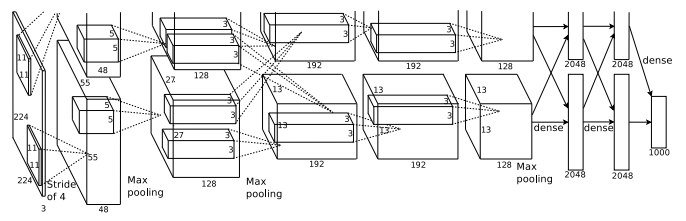
\includegraphics[width=\textwidth]{img/methods/alexnet_original.png}
	\caption{AlexNet architecture}
	\label{fig:alexnet_orig}
\end{figure}


\subsubsection{Training and testing}

We will be using the AlexNet as a source of inspiration for our network, with some minor tweaking as to fit our purpose. Note that the original design of the architecture was intended to be run in parallel on two GPUs, but as a first modification we will re-design it to be run sequentially on one.

Even though their potential for performing very well, one issue with ANNs is that they often require a lot of data to do so. The amount of data we have been able to gather by taking images of the objects are unfortunately not enough for a network as large as the AlexNet network. Fortunately for us there are pre-trained weights to be found that we can use as to increase our chances, for example we can use the ones found at \parencite{AlexNetImplWeights} where we can also base our implementation of the AlexNet architecture using the Python library \texttt{tensorflow}.

Next step is to finetune the pre-trained weights to better fit our own data. More precisely we will train it to output one of the labels created through the clustering instead one the one thousand classes it was originally trained for. As input data we will be taking inspiration from \parencite{Redmon2014} and to this with our own images but with the blue color channel replaced with the depth image.
